
%(BEGIN_QUESTION)
% Copyright 2012, Tony R. Kuphaldt, released under the Creative Commons Attribution License (v 1.0)
% This means you may do almost anything with this work of mine, so long as you give me proper credit

Calculate the {\it mechanical advantage} of this lever:

$$\includegraphics[width=15.5cm]{i02618x01.eps}$$

\underbar{file i02618}
%(END_QUESTION)





%(BEGIN_ANSWER)

For any lever -- regardless of class -- the mechanical advantage ($M_A$) is always calculated as the ratio of radii between the input and output points on the lever (i.e. the ratio of lengths -- also called ``moment arms'' -- between each point and the fulcrum).

In this case, since the ratio of moment arms lengths is 12:4 (3:1), the mechanical advantage will be 3:1 as well.  The person only needs to exert 1/3 the weight of the mass on the right-hand end of the lever in order to lift the mass, but the {\it motion} at that end of the lever will be three times as much as the motion of the mass.

%(END_ANSWER)





%(BEGIN_NOTES)


%INDEX% Machine, lever
%INDEX% Machine, mechanical advantage

%(END_NOTES)


